\section{Methoden und Durchführung}
\subsection{Kennlinie}
Zuerst soll die Kennlinie der Diode bestimmt werden. Dazu wird diese nach \cref{Aufbau} gemessen. Dabei wird die die Leistung der Mikrowellenstrahlung in Spannung umgewandelt. Dies wird auch in allen weiteren Messungen verwendet, da sich die Spannung einfacher direkt messen lässt.

\begin{figure}[h]
	\centering
	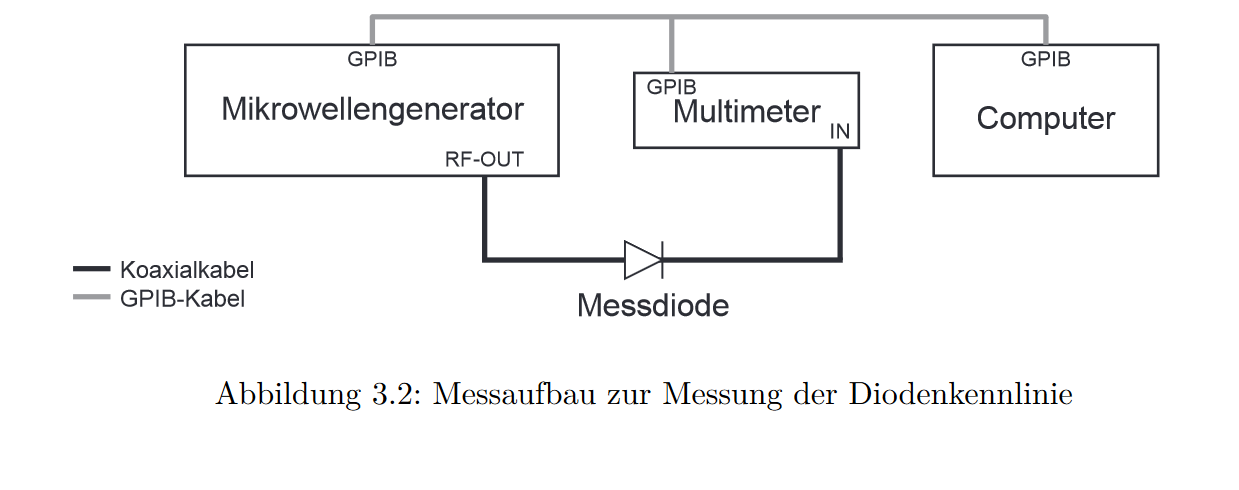
\includegraphics[scale=0.4]{Diode_Aufbau.PNG}
	\caption{Skizze des Versuchaufbaus}
	\label{Aufbau}
\end{figure}



\subsection{Zirkulator}
Ein Zirkulator ist ein Dreitor, welches eine stehende Welle nach dem Prinzip in \cref{ZB} weiterleitet.
\begin{figure}[h!]
	\centering
	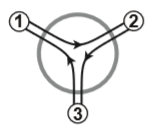
\includegraphics[scale = 1]{Zirk-Bild.PNG}
	\caption{}
	\label{ZB}
\end{figure}
Bei einem idealen Zirkulator geht der gesamte Stromfluss ohne Verlust  durch den Zirkulator hindurch. Somit tritt kein Energieverlust zwischen den Toren auf. Die gesamte Energie von Tor 1 tritt an Tor 2 aus. Analog der Pfeile tritt die gesamte Energie, die in Tor 2 bzw. in Tor 3 einläuft, bei Tor 3 bzw. bei Tor 1 aus. Wichtige Größen zur Charkterisierung des Zirkulators sind die Bandbreite, die Durchlassrichtung und die Sperrdämpfung.

\begin{align}
\text{Durchlassdämpfung} = 10 \cdot \ln{\frac{P_1}{P_2}}dB \\
\text{Sperrdämpfung} =  10 \cdot \ln{\frac{P_1}{P_3}}dB 
\end{align}

\subsection{Isolator}
Ein Isolator ist ein Zirkulator, welcher an Tor 3 ein angepassten Abschlusswiderstand besitzt. Das führt dazu, dass ein Isolator eine stehende Welle in eine Richtung nahezu durchlässt, wohingegen es den Strom in entgegengesetzter Richtung absorbiert. Sie werden genutzt um Mikrowellengeneratoren vor Reflexion zu schützen.

\subsection{Richtkoppler}
Ein Richtkoppler ermöglicht es Wellen mit verschiedenen Ausbreitungsrichtungen voneinander zu trennen. Das kann dazu dienen, dass man die einzelnen Wellen messen kann. Ein Richtkoppler ist ein Viertor. Analog zum Zirkulator besitzt es jedoch 4 Aus- bzw. Eingänge. Der schematische Aufbau eines Richtkopplers findet man in \cref{RB}. 
\begin{figure}[h!]
	\centering
	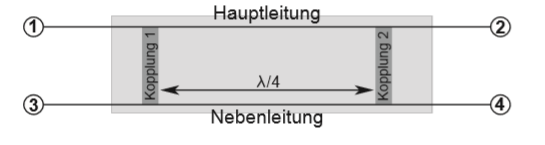
\includegraphics[scale = 1]{Richt-Bild.PNG}
	\caption{}
	\label{RB}
\end{figure}
Der Richtkoppler ist in eine Hauptleitung und in eine Nebenleitung eingeteilt. Er funktioniert über das Prinzip von konstruktiver und destruktiver Interferenz. Dazu werden die Haupt- und Nebenleitungen über einen Draht mit  einer Länge von $\frac{\lambda}{4}$ verbunden. Betrachten wir den Fall,dass eine Welle in Tor 1 ein läuft, so spaltet sich die Welle im ersten Kopplungspunkt in zwei Teilwellen auf. Einmal folgt die Welle der Hauptleitung und einmal wird diese auf die Nebenleitung übertragen. Bis die Welle die Nebenleitung erreicht, vergeht eine Länge von $\frac{\lambda}{4}$. Ebenso vergeht eine Länge von $\frac{\lambda}{4}$, bis die Welle den zweiten Kopplungspunkt auf der Hauptleitung erreicht. Hier spaltet sich die Welle wieder auf und benötigt wiederum eine Länge von $\frac{\lambda}{4}$ um die Nebenleitung zu erreichen. Wenn jetzt eine Welle von Tor 1 zu Tor 4 betrachtet wird, kann aufgrund von konstruktiver Interferenz ein Leistungsübertrag beobachtet werden, wohingegen bei einer Welle von Tor 1 zu Tor 3 eine destruktive Interferenz beobachtet wird. Das hängt damit zusammen, da die Welle im zweiten Fall genau eine Wellenlängenänderung von $\frac{\lambda}{2}$ erfährt.
Wie viel Leistung der Hauptleitung auf die Nebenleitung übertragen wird hängt von der Stärke der Kopplung ab. Sie wird durch die Koppeldämpfung beschrieben.
\begin{align}
\text{Koppeldämpfung} = 10\cdot \ln{\frac{P_1}{P_4}}dB
\label{KppF}
\end{align}
Die Isolation gibt an wie viel der Welle von Tor 1 ungewollt an Tor 3 ausgegeben wird.
\begin{align}
\text{Isolation} = 10\cdot \ln{\frac{P_2}{P_4}}dB
\label{IsoF}
\end{align}
Die Dämpfung auf der Hauptleitung gibt die Einfügedämpfung an. 
\begin{align}
\text{Einfügedämpfung} = 10\cdot \ln{\frac{P_1}{P_2}}dB
\label{EinF}
\end{align}
Um die Bauteile zu messen wird folgende Apparatur verwendet.
\begin{figure}[h!]
	\centering
	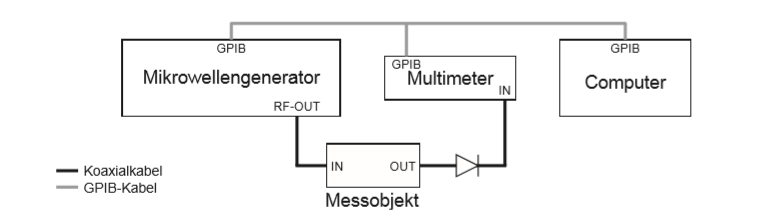
\includegraphics[scale = 1]{Mess.PNG}
	\caption{}
	\label{}
\end{figure}
Der Aufbau ähnelt dem vom vorherigen Versuch zur Bestimmung der Diodenkennnlinie. Jetzt wird ein Messobjekt zwischen dem Mikrowellengenerator und der Diode eingebaut. Zuerst betrachten wir ein Isolator, danach ein Zirkulator und zum Schluss einen Richtkoppler. Zum messen all dieser Bauteile wird ein vorprogrammiertes LabVIEW Programm benutzt. Dieses zeichnet die Spannung in Abhängigkeit von der Frequenz auf. Die Messwerte werden in Dämpfung pro Frequenz aufgetragen, sodass die folgende Umrechnung erfolgen muss, wobei P die Leistung darstellen soll.
\begin{align}
\text{dB} = 10\text{dBm} - \text{P}
\label{F1}
\end{align}

\subsection{Ausbreitungsgeschwindigkeit und relative Permittivität}
Zuletzt sollen in zwei verschiedenen Koaxialkabeln stehende Wellen erzeugt und die Resonanzfrequenzen, bei denen die stehenden Wellen beobachtet werden, gemessen werden. Aus den Abständen zwischen den Resonanzen soll anschließend mit \cref{eq:c} die Ausbreitungsgeschwindigkeit der Welle im Kabel berechnet werden.
\begin{equation}
c = 2l(f_{n+1} - f_n)
\label{eq:c}
\end{equation}
Zuletzt soll dann mit \cref{eq:er} die relative Permittivität bestimmt werden.
\begin{equation}
\epsilon_r = \left( \frac{c_0}{c}\right) ^2
\label{eq:er}
\end{equation}

\section{Auswertung}
\subsection{Kennlinie}
Zuerst wird die Kennlinie der Diode bestimmt. Diese wird in \cref{fuck_scidavis} dargestellt. Dabei wird mit einer e-Funktion gefittet, durch die beschrieben wird, welche Leistung in wie viel Spannung umgewandelt wird. 

\begin{figure}[h]
	\centering
	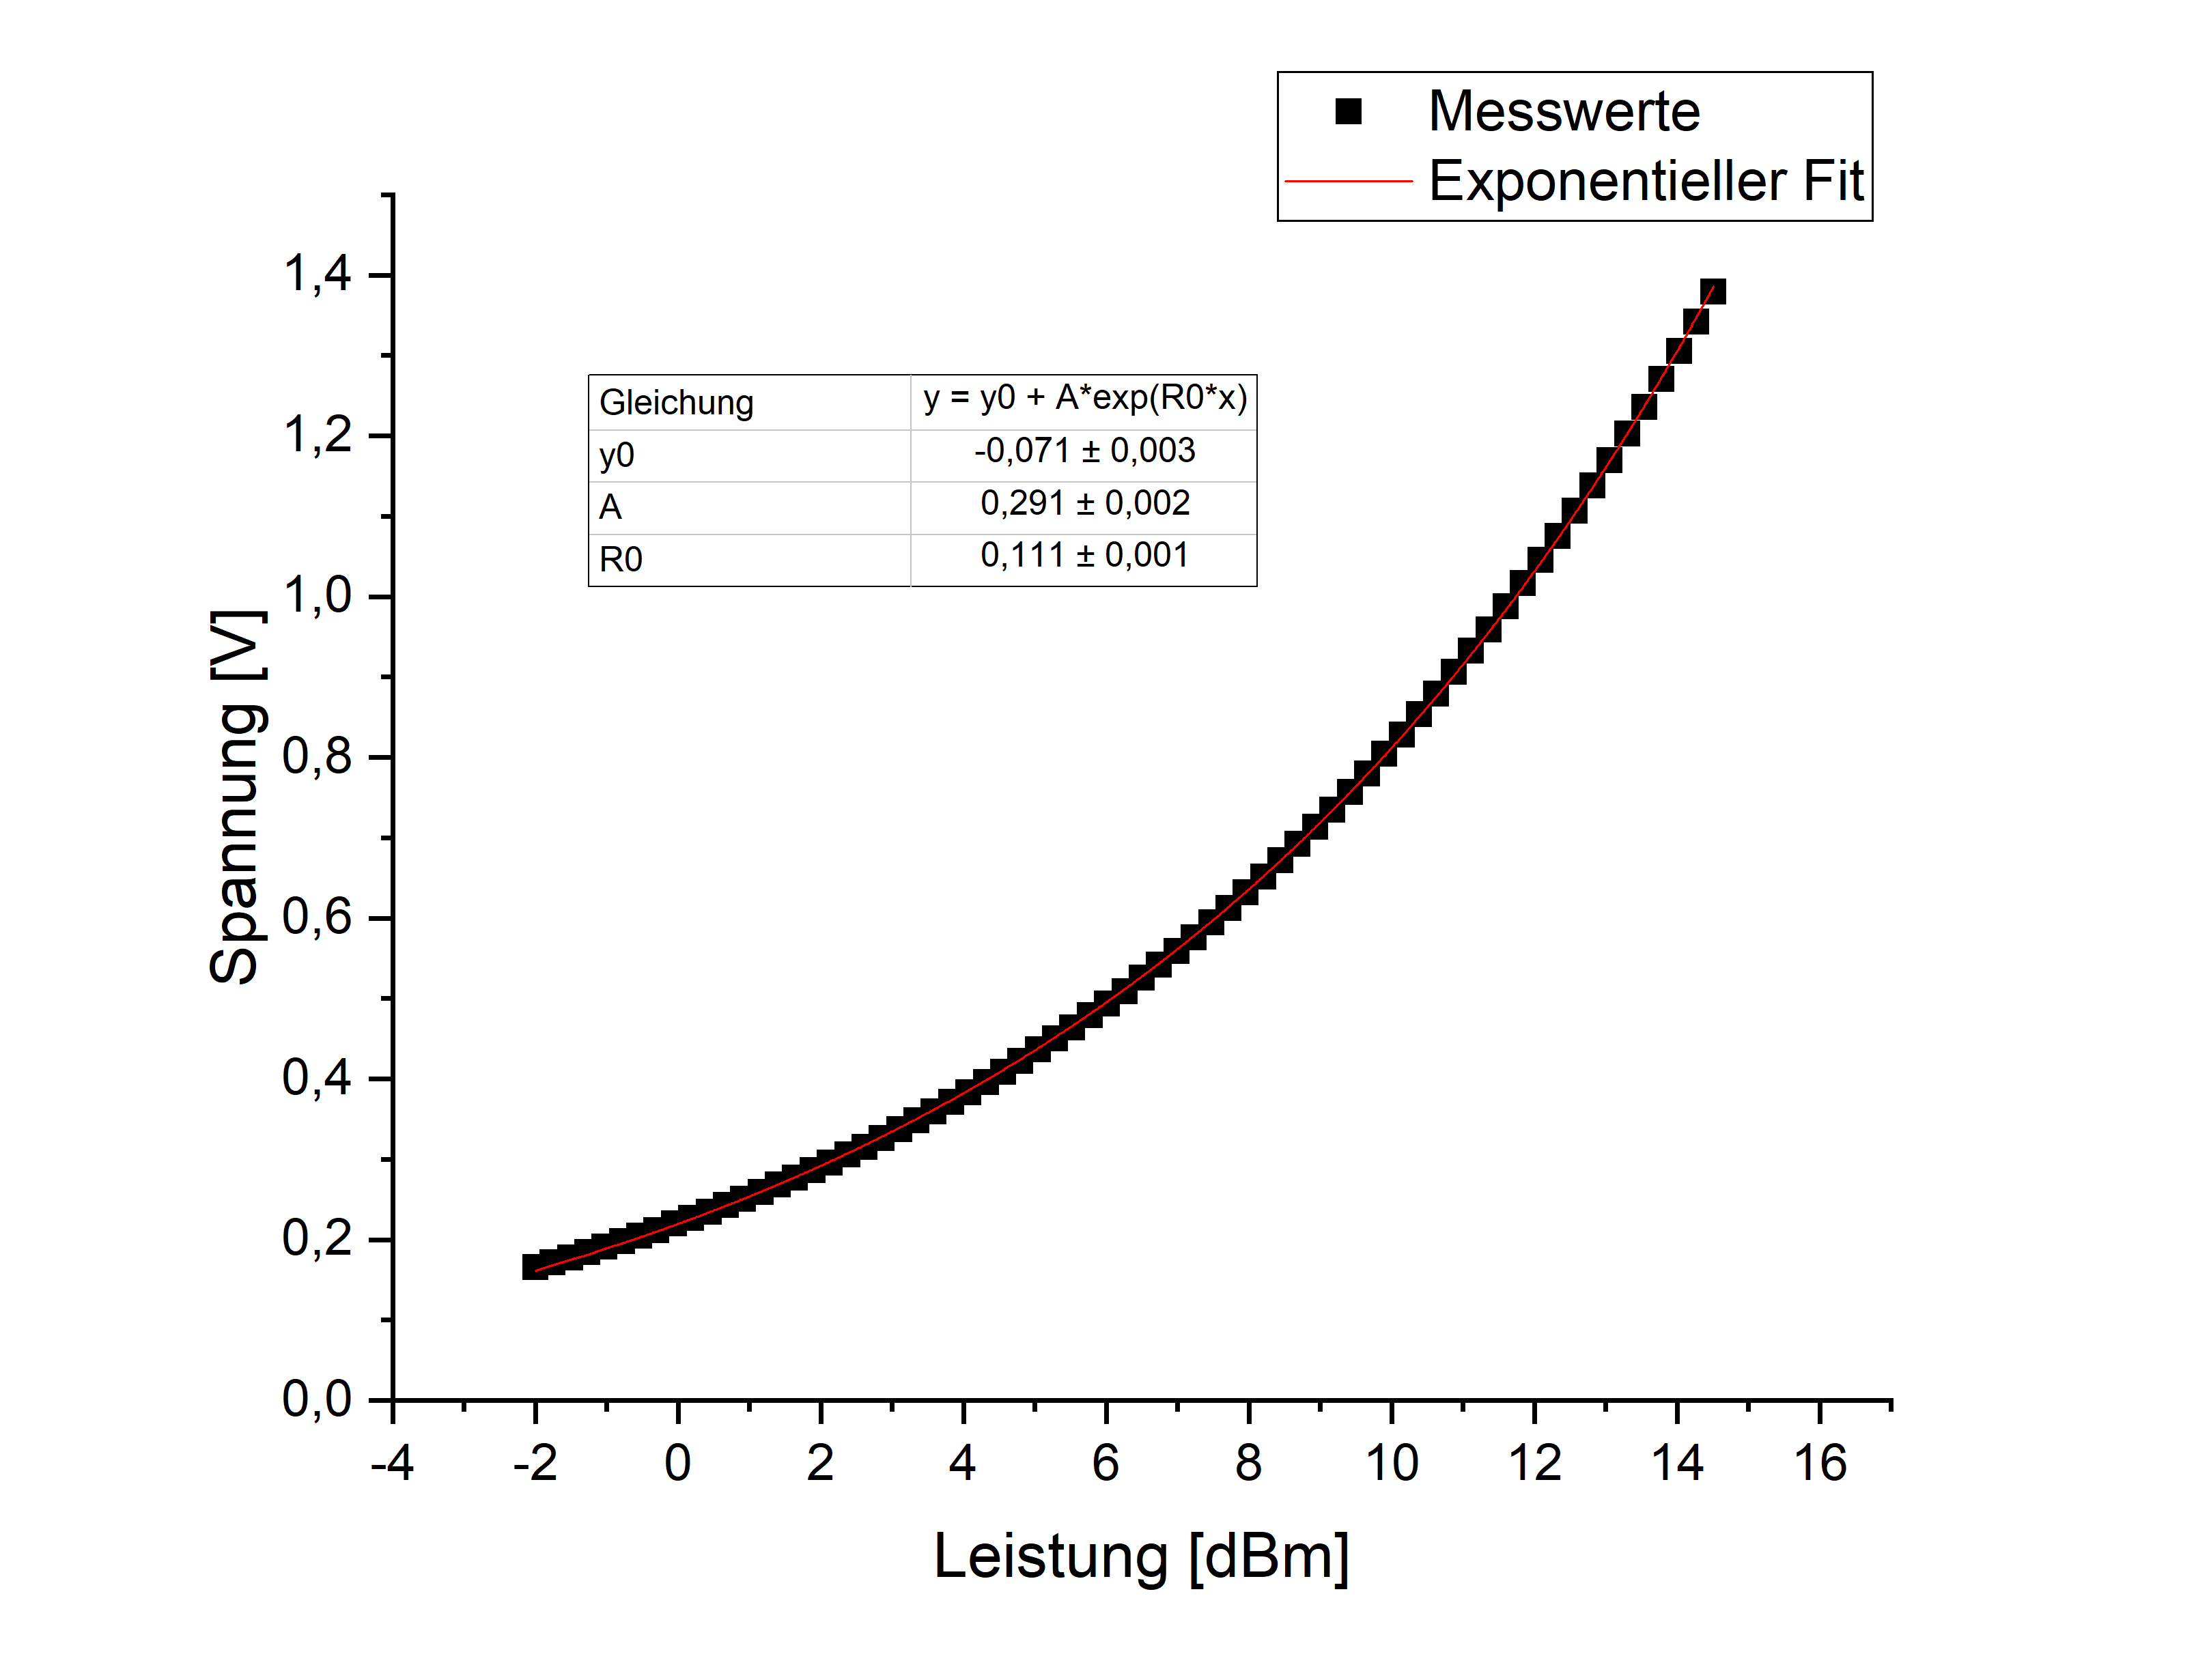
\includegraphics[scale=0.4]{fuck_scidavis.PNG}
	\caption{Kennlinie der Diode}
	\label{fuck_scidavis}
\end{figure}

\subsection{Bauteile der Hochfrequenztechnik}
In diesem Teil werden die Dämpfungen der Bauteile in Abhängigkeit der Frequenz dargestellt. Da in allen Messungen die Spannung in Abhängigkeit der Frequenz dargestellt wird, muss die Spannung zunächst mit der Formel der Diodenkennlinie in Leistung umgerechnet werden. Die Umrechnung von Leitung in Dämpfung erfolgt über \cref{F1}. Alle Grafiken wurden mit dem Programm OriginPro erstellt.
\subsubsection{Isolator}
in \cref{Isolator} ist die Dämpfung in abhängigkeit der Frequenz dargestellt. Wie erwartet besitzt die Sperrrichtung einen höheren Dämpfwert als die Durchlassrichtung. Innerhalb eines bestimmten Bereiches kann die Dämpfung als konstant angesehen werden außerhalb des Bereiches weißt die Kurve ein nicht lineares Verhalten auf. Es wird nur der Bereich charakterisiert, welcher ein nahezu lineares bzw. konstantes Verhalten aufweist.
\begin{figure}[h!]
	\centering
	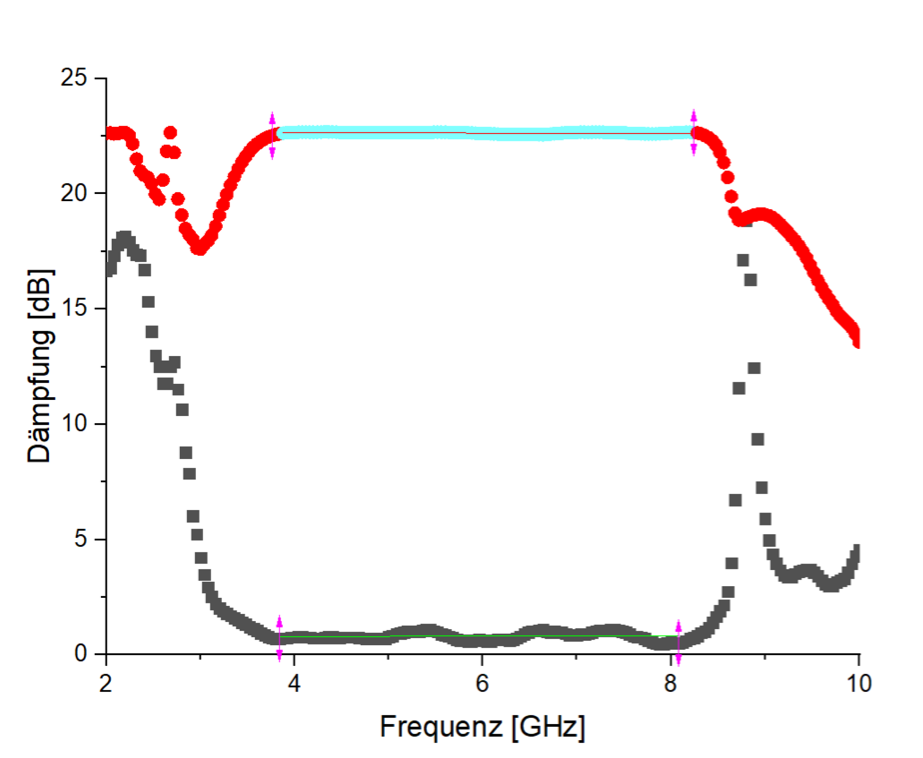
\includegraphics[scale = 1]{Isolator11.png}
	\caption{Die roten Punkte stellen die Sperrdämpfung dar. Das Intervall mit den türkisen Punkten stellt die Bandbreite sowie den ausgewerteten Bereich dar. Die schwarzen Punkte stellen die Durchlassdämpfung dar. Über die rosa Markierungen wurde der gefittete Bereich dargestellt. Dieser Bereich entspricht der Bandbreite. Die vorliegenden Fits entsprechen linearen Fits von der Form $y = a + bx$. Die Fitparameter in Sperrichtung sind $a = (22,70 \pm 0,02)$dB und $b = (-0,009 \pm 0,002)$dB/Ghz. Die Fitparameter in Durchlassrichtung betragen $a = (0,77 \pm 0,08)$dB und $b = (-0,01 \pm 0,01)$dB/GHz.}
	\label{Isolator}
\end{figure}
Die Bandbreite beider Dämpfungen befinden sich bei etwa 4Ghz bis 8Ghz. Bei der Durchlassdämpfung ist zu erkennen, dass die Steigung innerhalb der Messunsicherheiten Null betragen könnte, was auf den zu erwartenden konstanten Verlauf hinweisen würde, doch wenn man sich die Grafik genauer anschaut erkennt man bei der Durchlassdämpfung, dass sich Wellen innerhalb der Messwerte ausbilden. Diese Wellen können dadurch entstanden sein, dass der Draht der zwischen dem Mikrowellengenerator und dem Messobjekt befestigt worden ist relativ kurz war und eine starke Biegung an einer Stelle aufgewiesen hat. Genau an dieser Stelle konnte es bei einigen Frequenzen zur Reflexion kommen, sodass der Koaxialkabel ein Reflexionsanteil besessen hat, der sich negativ zum Durchlassvermögen auswirkte. Diese Ungenauigkeit wurde bei den flgenden Versuchen korrigiert, indem man ein längeres Kabel verbaut hat, welches keine starke Krümmung aufgewiesen hat. Bei der Sperrichtung ist ebenfalls ein nahezu konstanter Verlauf zu beobachten. Hier kann jedoch nicht innerhalb der Messunsicherheiten zu einem Konstanten Verlauf geschlossen werden. Die Steigung ist jedoch so gering, dass dies durch nicht berücksichtigte Unsicherheiten des Aufbaus zustande gekommen sein könnte. Mit Hilfe der Plots kann eine Dämpfung angegeben werden. Für die Durchlassrichtung beträgt die Dämpfung $a = (0,77 \pm 0,08)$ dB und die Dämpfung in Sperrichtung beträgt
$a = (22,70 \pm 0,02)$dB.

\subsubsection{Richtkoppler}
Als nächstes wird der Richtkoppler betrachtet. In \cref{Richt} ist die Isolation, die Koppeldämpfung und die Einfügedämpfung dargestellt. Dabei besitzt die Isolation die stärkste Dämpfung. Danach kommt die Koppeldämpfung und danach die Einfügedämpfung.
\begin{figure}[h!]
	\centering
	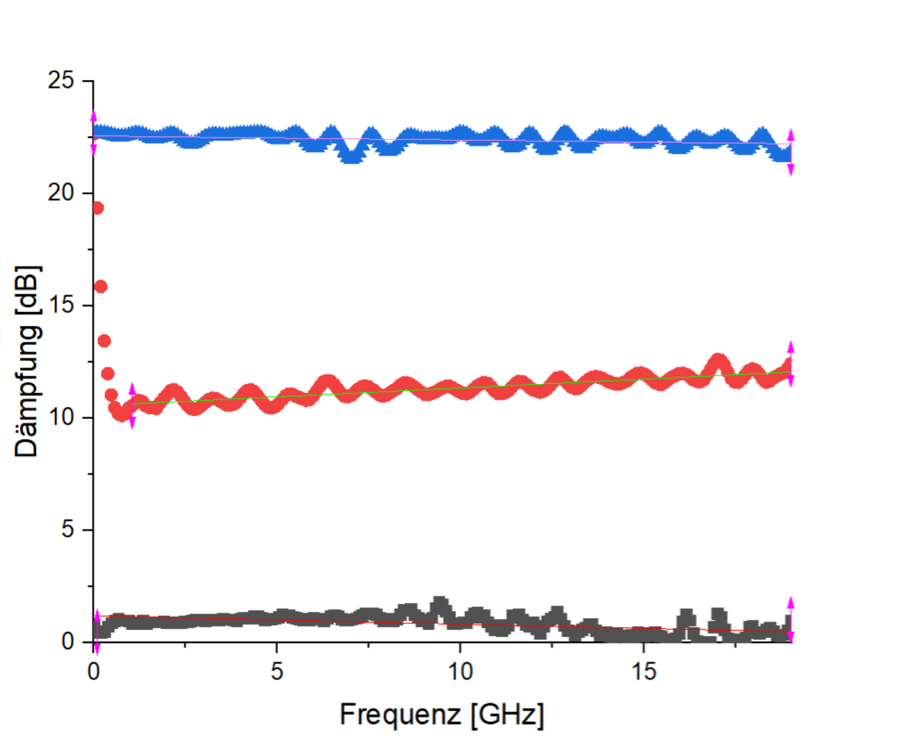
\includegraphics[scale = 1]{Richtkoppler11.png}
	\caption{In schwarz ist die Einfügedämpfung gemessen worden. Diese wurde mit dem orangen Fit mathematisch modelliert. Der Fit ist von der Form $y = a + bx$. Die Fitparameter sind $a = (1,20 \pm 0,04)$dB und $b = (-0,04 \pm 0,004)$dB/Ghz.
	In rot ist die Koppeldämpfung gemessen worden. Diese wurde mit dem grünen Fit mathematisch modelliert. Der Fit ist von der Form $y = a + bx$. Die Fitparameter sind $a = (10,55 \pm 0,04)$dB und $b = (-0,08 \pm 0,003)$dB/Ghz. Die senkrechten Markierungen stellen den Bereich dar, der Modelliert wird.
	In blau ist die Isolation gemessen worden. Diese wurde mit dem rosa Fit mathematisch modelliert. Der Fit ist von der Form $y = a + bx$. Die Fitparameter sind $a = (22,57 \pm 0,03)$dB und $b = (-0,02 \pm 0,003)$dB/Ghz.}
	\label{Richt}
\end{figure}
Auch bei dem Richtkoppler kann erkannt werden, dass die Dämpfung nahe zu konstant sind. Es ist zu beobachten, dass die Isolation die stärkste Dämpfung ist. Das ist deshalb so, da bei der Isolation die Wellen zu einer destruktiven Interferenz geführt werden, somit kann kaum Leistung übertragen werden. Dies ist der Fall, falls man die übertragene Leistung von Tor 2 zu Tor 4 misst, wie es in \cref{IsoF} steht.  Bei der Koppeldämpfung wird  die übertragenen Leistung von Tor 1 zu Tor 4 beobachtet (siehe \cref{KppF}). Hier ist die Dämpfung von Hauptleitung zu Nebenleitung zu sehen. Obwohl hier eine konstruktive Interferenz stattfindet, kommt es zur Dämpfung. Die Einfügedämpfung misst die Dämpfung der übertragenen Leistung von Tor 1 zu Tor 2. Da diese Strecke ohne jegliche Abzweigungen und Interferenzerscheinungen vonstatten geht, ist zu erwarten, dass hier die geringste Dämpfung stattfindet. Tatsächlich finden wir hier den geringsten Wert.

\subsubsection{Zirkulator}
Bei dem Zirkulator wurden zwei verschiedene Bauteile vermessen. Ein großer Zirkulator und ein kleiner Zirkulator. Beide Messkurven die des großen Zirkulators, sowie des kleinen Zirkulators wurde in Durch- und in Sperrrichtung vermessen und in einem Diagramm dargestellt.
\begin{figure}[h!]
	\centering
	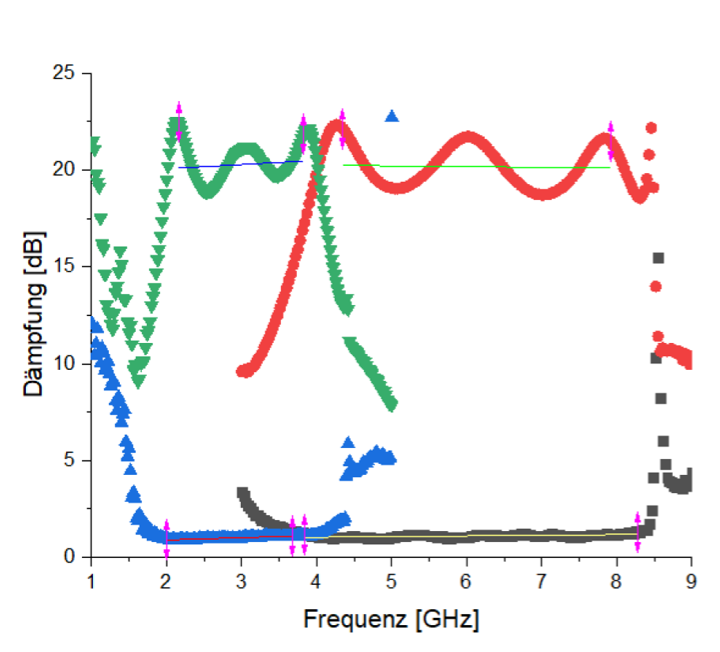
\includegraphics[scale = 1]{Zirkulator11.png}
	\caption{In diesem Bild können zwei Zirkulatoren beobachtet werden die schwarzen sowie die roten Punkte gehören dem kleinen Zirkulator. Die blauen und die grünen Dreiecke gehören zum großen Zirkulator. Die schwarzen und blauen Messwerte beschreiben die Durchlassrichtung und die roten und grünen Punkte die Sperrrichtung. Die senkrechten Markierungen stellen den gefitteten Bereich dar.
	Die jeweiligen Fits sind von der Form $y = a + bx$. 
	Die Durchlassrichtung des kleinen Zirkulators besitzen folgende Fitparameter ($a = (0,89 \pm 0,02)$dB und $b = (-0,03 \pm 0,004)$dB/Ghz.).
	Die Durchlassrichtung des großen Zirkulators besitzen folgende Fitparameter ($a = (0,65 \pm 0,02)$dB und $b = (-0,12 \pm 0,005)$dB/Ghz.).
	Die Sperrrichtung des kleinen Zirkulators besitzen folgende Fitparameter ($a = (20,4 \pm 0,6)$dB und $b = (0,65 \pm 0,02)$dB/GHz).
	Die Sperrrichtung des großen Zirkulators besitzen folgende Fitparameter ($a = (19,6 \pm 0,6)$dB und $b = (0,2 \pm 0,2)$dB/Ghz).}
	\label{ZirkB}
\end{figure}
In dem Diagramm sind zwei verschiedene Zirkulatoren zu sehen. Der heuristische Verlauf beider Graphen ist ähnlich. Beide Verläufe sind außerhalb der Bandbreiten der Sperrrichtung und Durchlassrichtung nicht linear. Innerhalb ihrer Bandbreiten stellen sich Resonanzen heraus, sodass diese sich nur im Mittel zu einer Konstanten ergeben. So stellt der geplottete Verlauf nur eine Näherung in nullter Ordnung dar und vernachlässigt die Dynamik innerhalb der Bandbreiten.
Die Bandbreite beträgt beim kleinen Zirkulator etwa 4GHz bis 8GHz und beim großen Zirkulator etwa 2GHz bis 3,7 GHz. Die einzigen Unterschiede in nullter Ordnung sind die, dass die Bauteile in verschiedenen Bandbreiten funktionieren und die Bandbreiten unterschiedlich groß sind. Die Bandbreite des kleinen Zirkulators ist dabei größer, als die des großen Zirkulators. Das Dämpfungsmaß ist hingegen bei beiden Zirkulatoren in Sperrichtung in Abhängigkeit der Fehler gleich groß und in Durchlassrichtung in Abhängigkeit der Fehler nur in derselben Größenordnung.

\subsection{Ausbreitungsgeschwindigkeit und relative Permittivität}
Im letzten Abschnitt werden Lichtgeschwindigkeit und Permittivität zwei verschiedener Koaxialkabel bestimmt. Zuerst wurde dafür der Abstand zwischen zwei benachbarten Resonanzen bestimmt. In \cref{gleich} sind die Messergebnisse für die Messung mit Kabel 1 sowohl für offenes Kabelende als auch für kurzgeschlossenes Kabelende dargestellt. Dabei ist die Leistung in dBm gegen die Frequenz in GHz aufgetragen.

\begin{figure}[h]
	\centering
	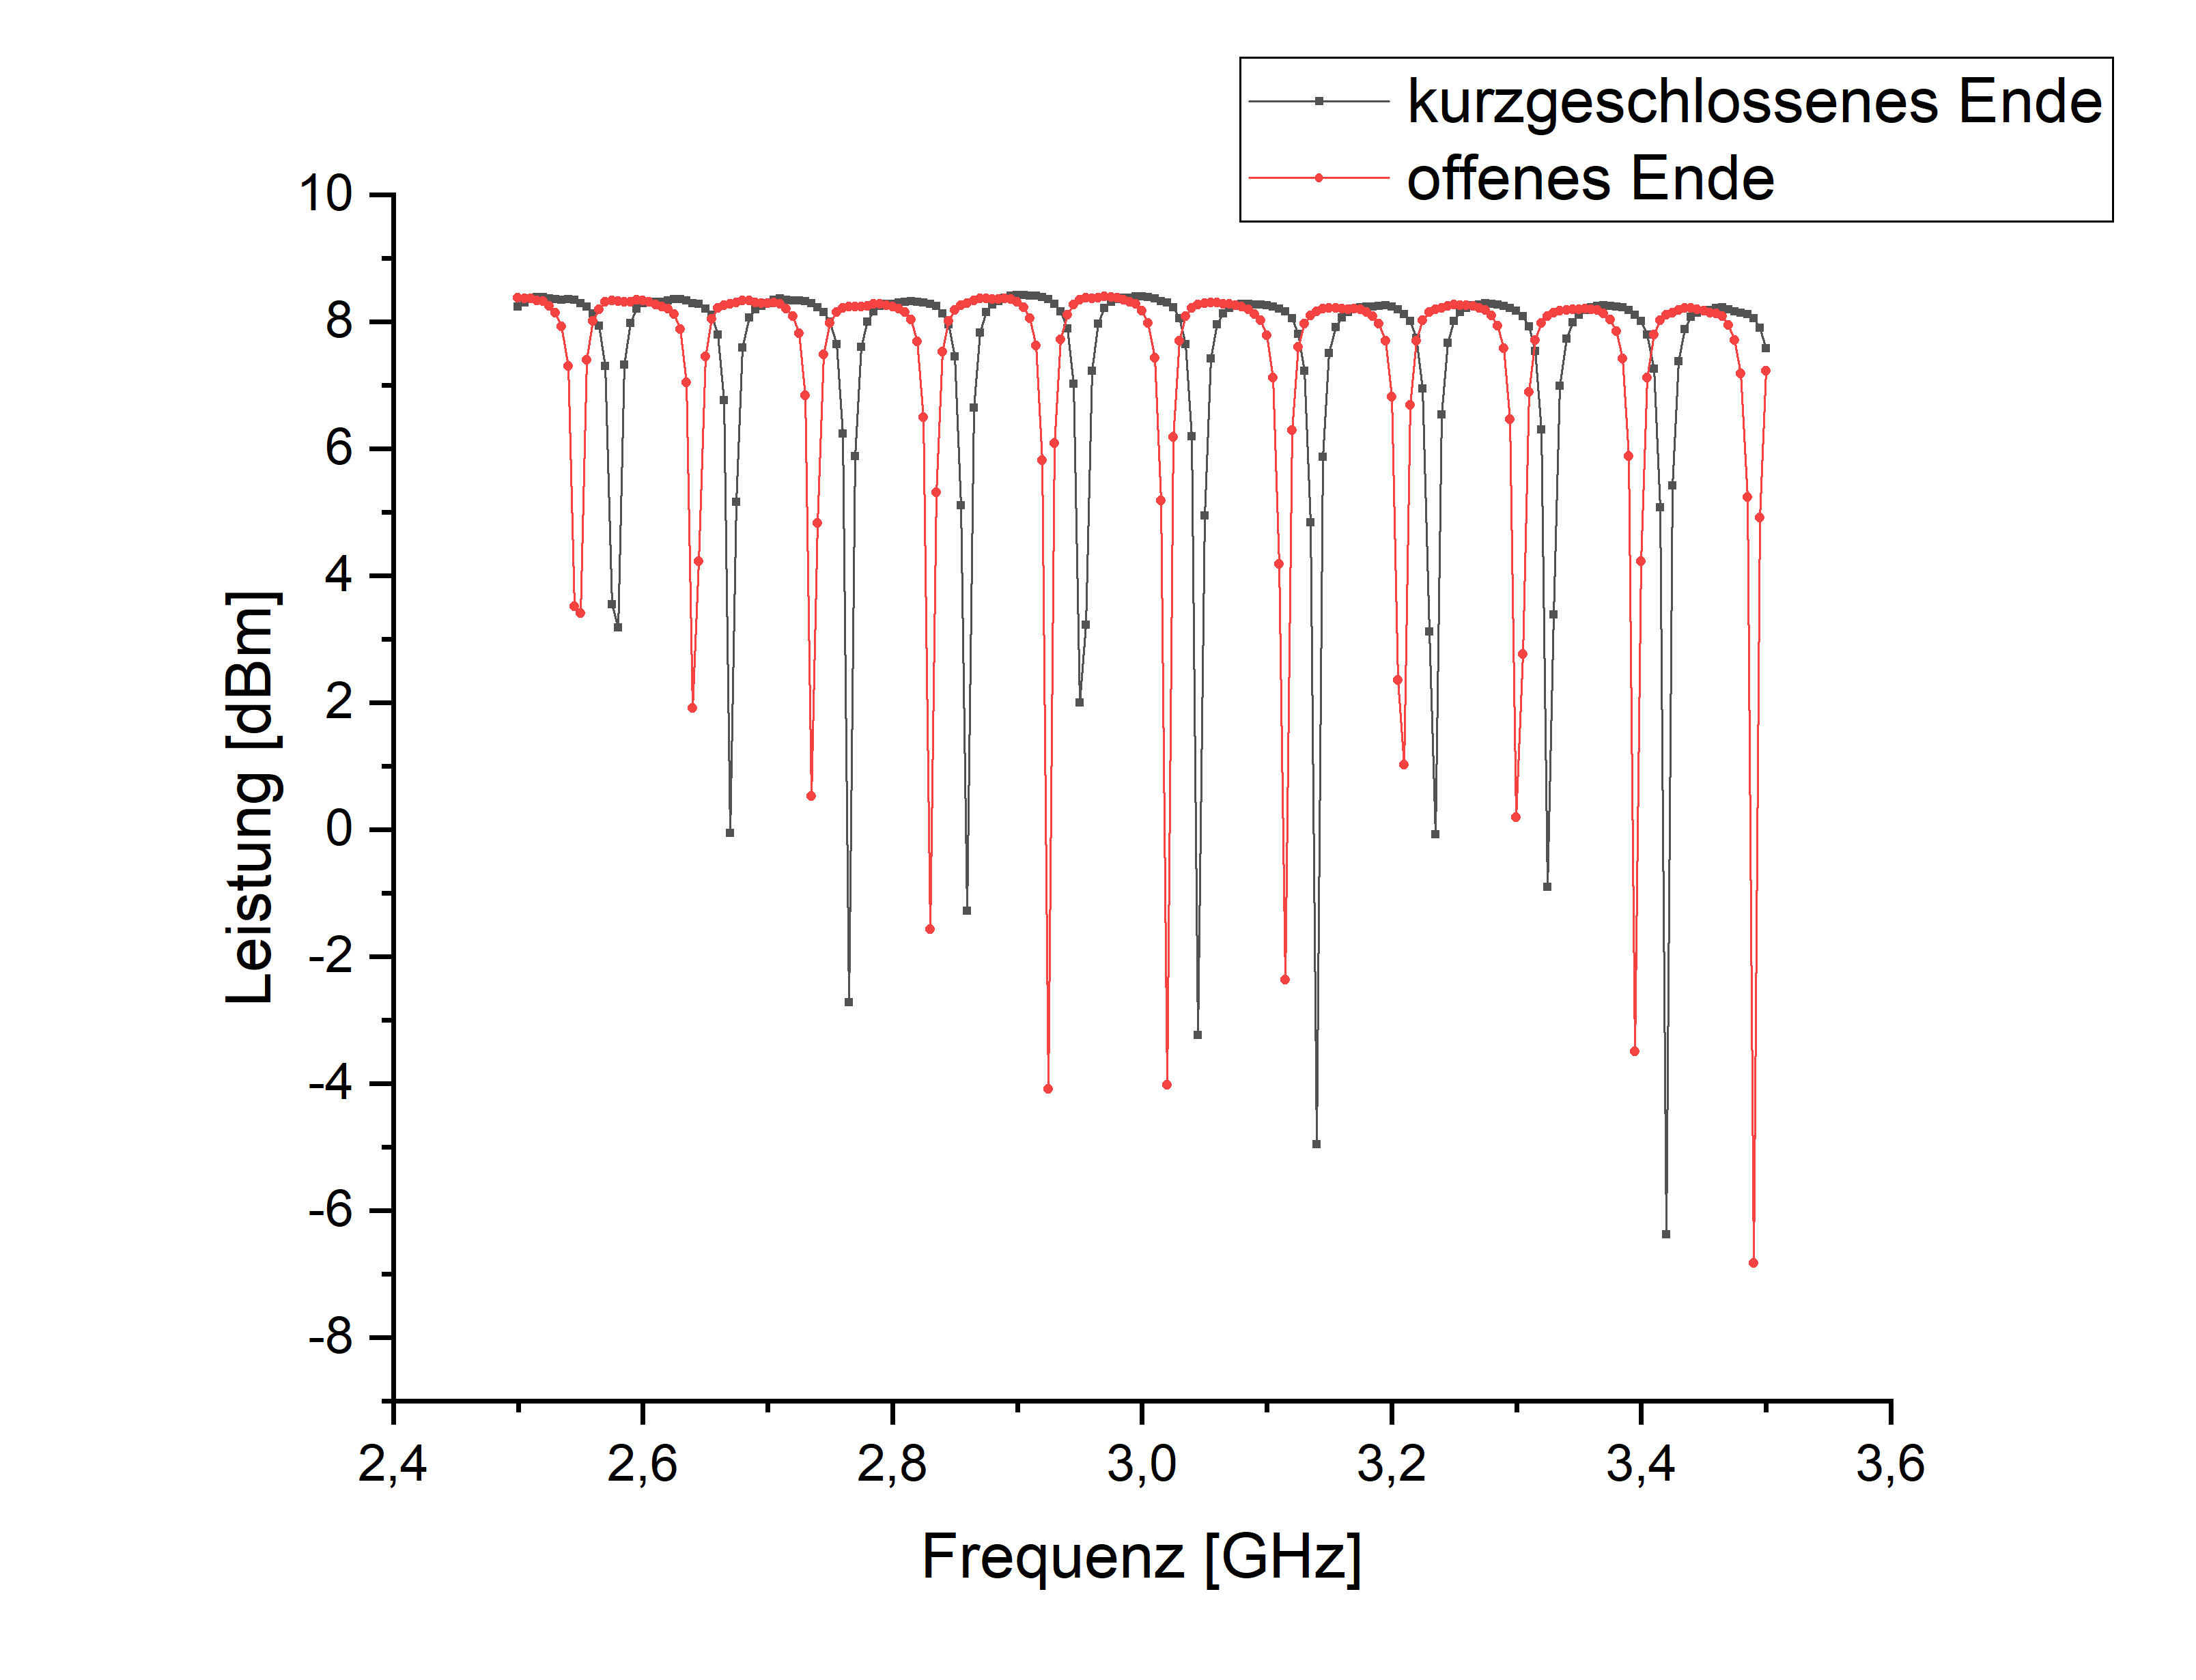
\includegraphics[scale=0.6]{gleiches_Kabel.png}
	\caption{Leistung in Abhängigkeit der Frequenz für offenes und kurzgeschlossenes Kabelende für Kabel 1. Deutlich erkennbar sind die Resonanzfrequenzen.}
	\label{gleich}
\end{figure}

Außerhalb der Resonanzen beträgt die Leistung konstant etwa $\SI{8}{dBm}$, an den Resonanzen fällt sie um mehrere Größenordnungen ab. Für beide Messungen wurde der mittlere Abstand zwischen zwei Resonanzfrequenzen ermittelt. Hierfür wurde der Mittelwert aus allen Frequenzabständen benachbarter Resonanzen gebildet.

\begin{figure}[h]
	\centering
	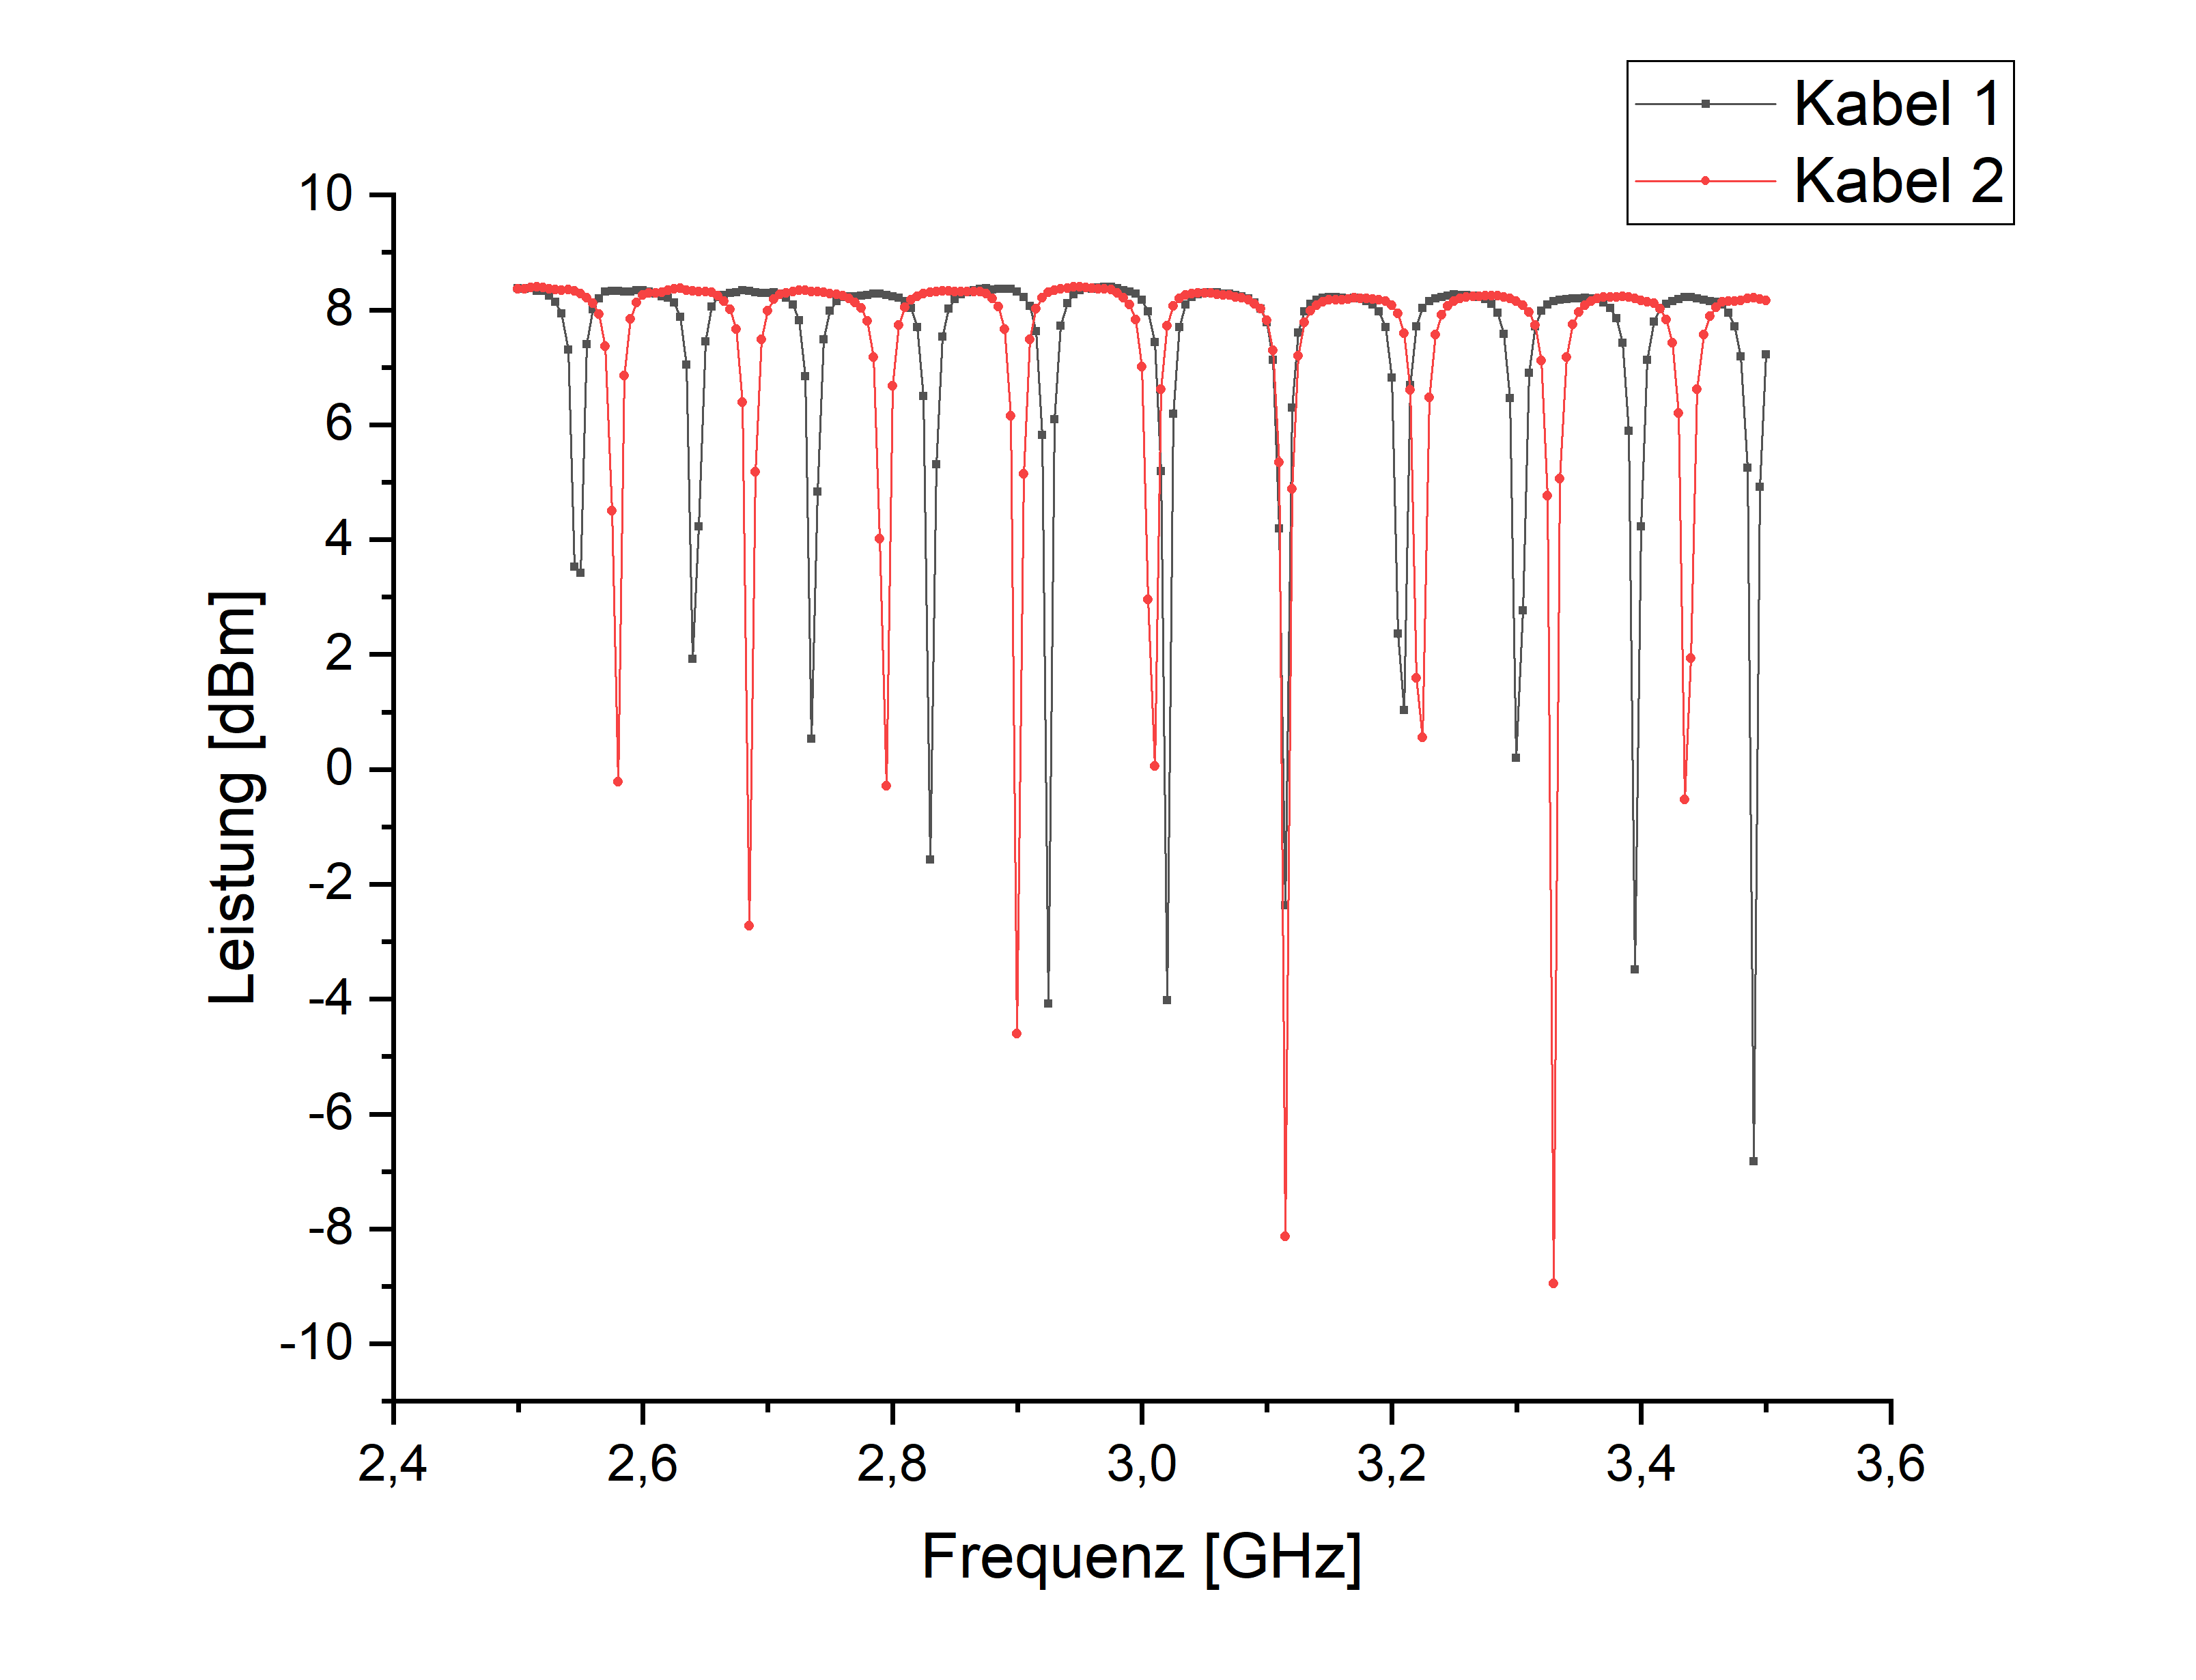
\includegraphics[scale=0.6]{anderes_Kabel.png}
	\caption{Leistung in Abhängigkeit der Frequenz für offenes Kabelende für Kabel 1 und 2. Deutlich erkennbar sind die unterschiedlichen Abstände zwischen den Resonanzen.}
	\label{anderes}
\end{figure}

Es ergeben sich Werte von $\SI{0,094\pm0,002}{GHz}$ für das offene Kabelende und $\SI{0,093\pm0,002}{GHz}$ für das geschlossene Kabelende. Die Unsicherheit ergeben sich aus direkt aus der Standardabweichung vom Mittelwert. Die Fehler der Geräte liegen unter $0,01\%$ und können daher vernachlässigt werden. Der mittlere Abstand der beiden Resonanzfrequenzen ist im Rahmen der Unsicherheit gleich. Die Art des Abschlusswiderstands hat damit offenbar keine Auswirkung auf den Abstand der Resonanzen. Allerdings treten die Resonanzen bei kurzgeschlossenem Ende jeweils bei um etwa $\SI{300}{MHz}$ höheren Frequenzen auf als die Resonanzen bei offenem Ende.

Für ein anderes Kabel (im folgenden Kabel 2) wurde anschließend die gleiche Messung mit offenem Ende durchgeführt. In \cref{anderes} werden die Ergebnisse der Messungen mit offenem Ende beider Kabel verglichen. Direkt erkennbar ist, dass hier der Abstand zwischen zwei Resonanzen unterschiedlich ist.


Auf die gleiche Weise wie oben wurde anschließend der mittlere Abstand zweier benachbarter Resonanzen bestimmt, hierfür ergibt sich ein Wert von $\SI{0,106\pm0,002}{GHz}$. Dieser ist signifikant größer als der von Kabel 1. Aus den mittleren Frequenzabständen kann nun mit \cref{eq:c} die Ausbreitungsgeschwindigkeit der Wellen im Koaxialkabel bestimmt werden. Die hierfür erforderliche Länge des Kabel wurde mit einem Maßband gemessen. Es ergibt sich für Kabel 1 bei offenem Ende ein Wert von $\SI{235000\pm5088}{km/h}$ und bei kurzgeschlossenem Ende ein Wert von $\SI{233333\pm5966}{km/h}$.Wie erwartet ist die Ausbreitungsgeschwindigkeit der Welle im Kabel unabhängig vom gewählten Abschlusswiderstand. Für Kabel 2 ergibt sich ein Wert von $\SI{254363\pm5859}{km/h}$. Die Unsicherheiten wurden über die Fehlerfortpflanzung mit \cref{eq:uc} berechnet.

\begin{equation}
	u(c) = \sqrt{\left( 2u(l)\Delta f\right) ^2 +\left( 2u(\Delta f)l\right) ^2}
	\label{eq:uc}
\end{equation}

Mithilfe der Ausbreitungsgeschwindigkeit kann nun über \cref{eq:er} die relative Permittivität bestimmt werden. Diese beträgt für Kabel 1 $\SI{1,627\pm0,070}{}$ bei offenem Ende bzw. $\SI{1,651\pm0,084}{}$. Es besteht also auch hier kein Unterschied bei verschiedenen Abschlusswiderständen. Für Kabel 2 beträgt die relative Permittivität $\SI{1,389\pm0,064}{}$. Die Unsicherheit wurde mit \cref{eq:uer} bestimmt.

\begin{equation}
	u(\epsilon_r) = \frac{2u(c)c^2}{c^3}
	\label{eq:uer}
\end{equation}

\section{Diskussion}
Wie erwartet war sowohl der Frequenzabstand zwischen zwei Resonanzen, als auch die Ausbreitungsgeschwindigkeit und die relative Permittivität unabhängig von der Wahl des Abschlusswiderstands. Dieser sorgte nur für eine Verschiebung der Resonanzen um einige $100$ MHz. Da die beiden Kabel unterschiedliche Ausbreitungsgeschwindigkeiten und relative Permittivitäten besitzen, bestehen sie offenbar aus unterschiedlichen Stoffen oder eins der Kabel ist beschädigt oder verunreinigt.